\chapter{Product development}
This chapter describes the technical side of this project. The technologies used, the network peripherals and the architecture of the iCare system are discussed here.

\section{Mocks}

\section{Implementation - Frontend}

The frontend was implemented with HTML, CSS and Javascript (ES6).
The following open source libraries were used:
\begin{itemize}

\item Chart.js to -  draw the diagrams in the Eco Monitor.
\item Date.js - to manipulate and format dates.
\item P5.js - to draw the interactive tracking interface.
\item Bootstrap 3 - a CSS framework to ensure a modern responsive user interface.
\end{itemize}


The focus in the design was placed on displaying the important messages (alarms) on each page so that staff can always see which new alarms have just been reported.
The user must manually mark these messages as read so that these messages are no longer displayed in the upper right-hand corner. For testing purposes during development, a Develop Tools page was implemented to manually force certain events to test the frontend end-to-end.

\subsection{Dynamic website}
Through timers the frontend calls the backend in the background at regular intervals (1 second), this ensures that the data in the frontend is always up-to-date.

\subsection{Tracking page}
On this page you can see a floor plan of the building showing the positions of the tracked inhabitants.
Every second the points are updated and the corresponding data is updated.
By clicking on a point, the current values of this inhabitant are displayed below the building floor plan ( Heart rate, Health Check, Restrictions, Name and ID).
The colors of the point have been implemented in a traffic light scheme. The dots on the floor plan, each representing an inhabitant, are displayed in these colors accordingly.


\subsection{Dashboard / Notifications}

This page lists the latest notifications in the system in chronological order. 
At the top of the screen, the user also sees additional counters for the various categories: Messages, alerts, tickets and todos. If the user clicks on one of these four fields, a corresponding page appears, which displays the data in more detail.
It was important that an appropriate colour scheme was consistently followed.
Red means urgent information. Yellow, a warning that is not quite as urgent and green means information.
Each notification contains a time stamp, a message, a room in which the event occurred, and the inhabitant, if any.

\subsection{Notification popup}

When a specific event occurs, notifications are sent to the frontend. If the frontend receives a new message, it is stored in an inbox in the frontend. The number of unread notifications is displayed as a red box in the upper right corner of each page of iCare. As soon as at least one unread notification is in the inbox, this red box is displayed. This ensures that important messages do not appear only once and are then missed by the user.
Clicking on this popup takes the user to an overview page in which all unread notifications are listed. With one button, he can set all these messages to read. After that the inbox is empty and the red box is no longer displayed until a new notification arrives.
If notifications are removed from the inbox, they are not deleted, but are still displayed in the recent list in the dashboard.


\subsection{Eco Monitor}

This page provides an overview of the electricity and water consumption of the last 30 days.
In this case, the data is only loaded once when the web page is loaded, since this data does not change as frequently.



\subsection{Camera page}

This page shows the user the last images of the surveillance cameras installed in the Carehome.
At the top he sees the pictures from the reception hall and below the pictures from the outside area. Additionally, a timestamp is diplayed to indicate when the image was taken.

\subsection{Report page}

This page allows you to generate a report for a specified period of time and download it as a pdf file.
The report includes water and electricity consumption. As well as a record of each resident's health check sensors.


\subsection{Settings page}
This page allows you to configure certain settings on the frontend.


\section{Basic architecture}
In order to give the user as much freedom as possible and to save him the installation and administration of unnecessary software and unnecessary software components, this project is implemented as a web server. This means that the system can be accessed by every employee under their user ID and password via the Internet using a web browser. The user interface elements are designed to be comfortably operated from a desktop PC as well as from mobile devices such as tablets and smartphones. This makes the iCare system platform independent and supports an easy and elegant user experience. The intention is to make it as easy as possible for the user to use the iCare system by using technologies that every user can use intuitively.

\subsection{iCare Network}
The server uses both wireless connections and the Ethernet connection within the care home to communicate with all connected devices as well as the backup system. As already described in chapter \ref{basic-concept}, each room within the care home has a network HUB, which is connected to the central server via Ethernet. This network HUB communicates either via an Ethernet connection or via a wireless connection with the devices installed in the room. Figure \ref{icare-network} shows the network peripherals of the iCare system:
\begin{figure}[H]
	\centering
	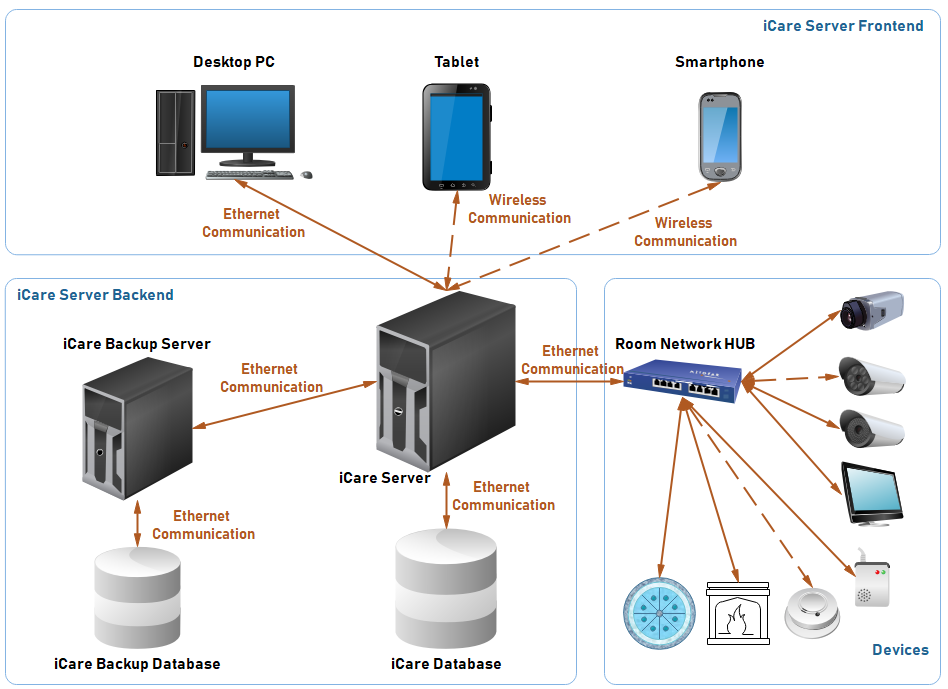
\includegraphics[width =1.0\textwidth]{images/iCare-Network.PNG}
	\caption{iCare Network}
	\label{icare-network}
\end{figure}
The solid lines represent communication via Ethernet cabling, while the dashed lines indicate a wireless connection. The devices connected to the network HUB are already listed in the overview in chapter \ref{basic-concept} for each room and are not considered here. A detailed examination of the individual devices can be found in the hardware calculation in Chapter \ref{market-analysis}.

\subsection{iCare Communication}
The data collected by the devices in the individual rooms is forwarded to the central server via the network HUB. The server analyzes this data, persists it in the database, forwards it to the backup system, and prepares it for display in the frontend of the iCare system. The processed data will also be forwarded to the infoboard for presentation via the network hub of the community room. It is also possible to access and control the devices for central heating and water consumption via the network HUB. For the frontend, it is also possible to send user inputs and user requests to the central server at any time, which then processes them and returns the corresponding results to the frontend. These data and control flows are shown in figure \ref{icare-dataflow}.
\begin{figure}[H]
	\centering
	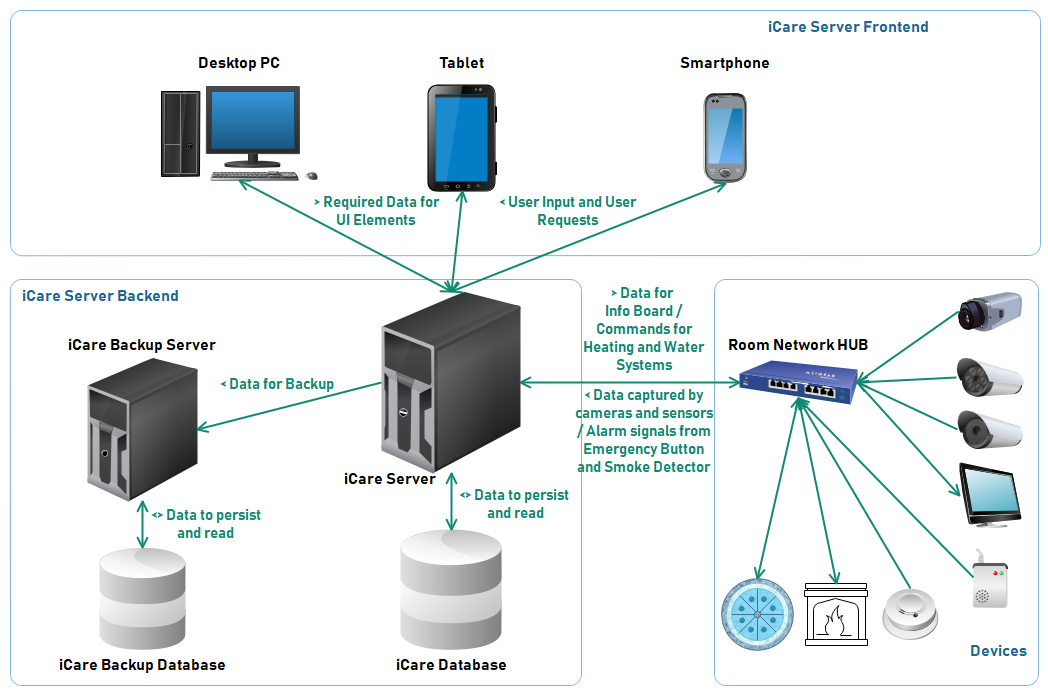
\includegraphics[width =1.05\textwidth]{images/iCare-Dataflow.PNG}
	\caption{iCare control- and data- flows}
	\label{icare-dataflow}
\end{figure}

A more detailed description of the individual subsystems will be given in the next chapters. It focuses on how the communication between the frontend and the backend of the iCare server is implemented, which data model is used, and which features the server offers the user.
